\documentclass[aspectratio=169, 11pt]{beamer}
\usetheme{default}

% Packages
\usepackage[utf8]{inputenc}
\usepackage{amsmath, amssymb, amsfonts}
\usepackage{booktabs}
\usepackage{tikz}
\usetikzlibrary{shapes.geometric, arrows.meta, positioning, calc}
\usepackage{hyperref}

% Premium Color Scheme (Academic Light Theme)
\definecolor{bglight}{RGB}{255, 255, 255}
\definecolor{textdark}{RGB}{30, 41, 59}       % Slate 800
\definecolor{primary}{RGB}{30, 58, 138}       % Deep Navy
\definecolor{secondary}{RGB}{37, 99, 235}     % Royal Blue
\definecolor{accentpink}{RGB}{190, 24, 74}    % Rose 700 (Academic Crimson)
\definecolor{accentgreen}{RGB}{4, 120, 87}    % Emerald 700

% Apply Light Theme Colors to Beamer
\setbeamercolor{background canvas}{bg=bglight}
\setbeamercolor{normal text}{fg=textdark}
\setbeamercolor{structure}{fg=primary}
\setbeamercolor{title}{fg=primary}
\setbeamercolor{subtitle}{fg=textdark!80}
\setbeamercolor{author}{fg=textdark!80}
\setbeamercolor{date}{fg=textdark!60}

% Header and Title Customization
\setbeamercolor{frametitle}{fg=primary, bg=bglight}
\setbeamerfont{title}{size=\Large, series=\bfseries}
\setbeamerfont{frametitle}{size=\large, series=\bfseries}

% Remove default navigation symbols
\setbeamertemplate{navigation symbols}{}

% Simple Footer
\setbeamertemplate{footline}{
    \leavevmode%
    \hbox{%
        \begin{beamercolorbox}[wd=.5\paperwidth,ht=2.25ex,dp=1ex,left,leftskip=1.5cm]{page number in head/foot}%
            \usebeamerfont{page number in head/foot}\color{textdark!60}A Geometric and Bayesian Formulation of LLMs
        \end{beamercolorbox}%
        \begin{beamercolorbox}[wd=.5\paperwidth,ht=2.25ex,dp=1ex,right,rightskip=1.5cm]{page number in head/foot}%
            \usebeamerfont{page number in head/foot}\color{textdark!60}\insertframenumber{} / \inserttotalframenumber
        \end{beamercolorbox}%
    }%
    \vskip0pt%
}

% Block Environments Customization (Clean Academic Blocks)
\setbeamercolor{block title}{bg=primary!10!bglight, fg=primary}
\setbeamercolor{block body}{bg=white!95!primary, fg=textdark}
\setbeamercolor{block title example}{bg=secondary!10!bglight, fg=secondary}
\setbeamercolor{block body example}{bg=white!95!secondary, fg=textdark}

% Slide Information
\title{A Geometric and Bayesian Formulation of Autoregressive Language Models}
\author{Akshay Mishra}
\date{\today}

\begin{document}

% Slide 1: Title Slide
\begin{frame}[plain]
    \centering
    \vfill
    \begin{minipage}{\textwidth}
        \centering
        \vspace{1cm}
        {\usebeamerfont{title}\color{primary}\inserttitle}\\[0.4cm]
        {\color{primary!80}\hrule height 1.5pt}\vspace{0.4cm}
        {\color{textdark!85}\large Decomposing Causal Paths, Latent Stream Variance, and Pre-Training Forces}\\[0.8cm]
        {\color{secondary}\insertauthor}\\[0.2cm]
        {\color{textdark!60}\small Research Presentation}
    \end{minipage}
    \vfill
\end{frame}

% Slide 2: The Bayesian Framing
\begin{frame}{1. The Bayesian Formulation of Language Modeling}
    \begin{columns}[T]
        \begin{column}{0.55\textwidth}
            Autoregressive models compute the next-token probability $P(w \mid C)$ directly. We invert this via Bayes' Theorem to expose the generative mechanics~\cite{jaynes1957}:
            \begin{block}{Bayesian Decomposition}
                $$P(w \mid C) = \frac{P(C \mid w) \cdot P(w)}{P(C)} \propto P(C \mid w) \cdot P(w)$$
            \end{block}
            \vspace{0.2cm}
            Where:
            \begin{itemize}
                \item \color{secondary} $P(w)$ \color{textdark} is the \textbf{unconditional token prior} (language baseline).
                \item \color{accentpink} $P(C \mid w)$ \color{textdark} is the \textbf{contextual likelihood} (context match).
            \end{itemize}
        \end{column}
        
        \begin{column}{0.4\textwidth}
            \centering
            \vspace{0.5cm}
            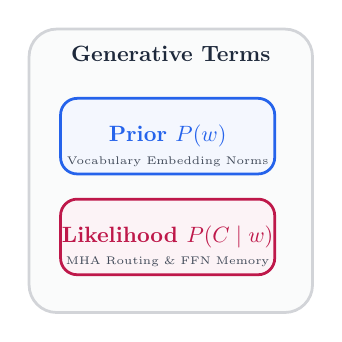
\begin{tikzpicture}[scale=0.8, every node/.style={transform shape}]
                % Bayes Box
                \draw[draw=textdark!20, fill=textdark!2, rounded corners=10pt, line width=1pt] (0,0) rectangle (4.5,4.5);
                \node at (2.25, 4.1) [color=textdark, font=\bfseries] {Generative Terms};
                
                % Prior Box
                \draw[draw=secondary, fill=secondary!5, rounded corners=6pt, line width=1pt] (0.5, 2.2) rectangle (3.9, 3.4);
                \node at (2.2, 2.8) [color=secondary, font=\bfseries] {Prior $P(w)$};
                \node at (2.2, 2.4) [color=textdark!85, font=\tiny] {Vocabulary Embedding Norms};
                
                % Likelihood Box
                \draw[draw=accentpink, fill=accentpink!5, rounded corners=6pt, line width=1pt] (0.5, 0.6) rectangle (3.9, 1.8);
                \node at (2.2, 1.2) [color=accentpink, font=\bfseries] {Likelihood $P(C \mid w)$};
                \node at (2.2, 0.8) [color=textdark!85, font=\tiny] {MHA Routing \& FFN Memory};
            \end{tikzpicture}
        \end{column}
    \end{columns}
\end{frame}

% Slide 3: Multi-Head Attention as Contextual Routing
\begin{frame}{2. Likelihood: Multi-Head Attention as Contextual Routing}
    In layer $l$, the MHA block computes token-to-token dependencies. For head $g \in \{1,\dots,H\}$ with key-query dimension $d_k$, the routing weights $\alpha_{n,i}^{(l,g)}$ align the terminal query with preceding keys~\cite{vaswani2017attention}:
    \begin{block}{Attention Routing \& Likelihood Contribution}
        $$\alpha_{n,i}^{(l,g)} = \frac{\exp\left(\frac{q_n^{(l,g)} \cdot k_i^{(l,g)}}{\sqrt{d_k}}\right)}{\sum_{j=1}^n \exp\left(\frac{q_n^{(l,g)} \cdot k_j^{(l,g)}}{\sqrt{d_k}}\right)}$$
        $$\log P(C \mid w)_{\text{MHA}} \sim \sum_{g=1}^H \sum_{i=1}^n \alpha_{n,i}^{(l,g)} \left( h_i^{(l-1)} W_V^{(l,g)} W_{O,g}^{(l)} u_w \right)$$
    \end{block}
    This separates dynamic context routing ($\alpha_{n,i}^{(l,g)}$) from semantic value alignment ($h_i W_V W_{O,g} u_w$).
\end{frame}

% Slide 4: Feed-Forward Networks as Concept Memory Retrieval
\begin{frame}{3. Likelihood: FFN as Concept Memory Retrieval}
    The position-wise Feed-Forward Network (FFN) functions as a key-value associative memory over conceptual rules, mapping context to target tokens~\cite{geva-etal-2021-transformer}:
    \begin{block}{FFN Associative Memory \& Likelihood Contribution}
        $$\text{FFN}(x_n^{(l)}) = \sum_{m=1}^{d_{ff}} \sigma\left( x_n^{(l)} \cdot k_m^{(l)} + b_{1,m}^{(l)} \right) v_m^{(l)}$$
        $$\log P(C \mid w)_{\text{FFN}} \sim \sum_{m=1}^{d_{ff}} \sigma\left( x_n^{(l)} \cdot k_m^{(l)} + b_{1,m}^{(l)} \right) \cdot (v_m^{(l)} \cdot u_w)$$
    \end{block}
    where $\sigma(\cdot)$ measures the scale of \textbf{rule satisfaction} for concept $m$, and $(v_m^{(l)} \cdot u_w)$ represents the \textbf{concept-to-token semantic alignment}.
\end{frame}

% Slide 5: Unembedding Bias and Norms as the Prior
\begin{frame}{4. Prior: Unembedding Bias and Vector Norms}
    The unconditional token prior $P(w)$ is stored statically within two parameters during optimization:
    \begin{columns}[T]
        \begin{column}{0.5\textwidth}
            \begin{block}{1. Unembedding Bias ($b_{U,w}$)}
                In models featuring explicit unembedding bias, under an uninformative context ($h_n \to \mathbf{0}$), the prior is:
                $$P(w) \approx \frac{\exp(b_{U,w})}{\sum_{v \in V} \exp(b_{U,v})}$$
            \end{block}
        \end{column}
        \begin{column}{0.5\textwidth}
            \begin{block}{2. Embedding Vector Norms ($\|u_w\|$)}
                Decomposing the logit $z_w = h_n^{(L)} \cdot u_w$ geometrically yields~\cite{gao2019representation}:
                $$z_w = \|h_n^{(L)}\| \|u_w\| \cos(\theta_w)$$
                High baseline frequencies in the corpus drive the vector magnitude $\|u_w\|$ upward, acting as a context-free prior booster.
            \end{block}
        \end{column}
    \end{columns}
\end{frame}

% Slide 6: Statistical Mechanics & Inverse Temperature
\begin{frame}{5. Statistical Mechanics: Latent Stream Variance}
    The norm of final hidden state $\|h_n^{(L)}\|$ acts as a context-dependent entropy controller:
    \begin{block}{Activation Variance to Vector Magnitude}
        If cross-channel mean is centered near zero ($\mu_x \approx 0$)~\cite{ba2016layernorm}:
        $$\|h_n\| = \sqrt{d \cdot \sigma^2}$$
    \end{block}
    This maps to the physical \textbf{inverse temperature} $\beta = \frac{1}{T}$ in Softmax~\cite{jaynes1957, ackley1985learning}:
    $$P(w \mid C) = \frac{\exp\big(\beta \cdot \|u_w\| \cos(\theta_w)\big)}{\sum_{v \in V} \exp\big(\beta \cdot \|u_v\| \cos(\theta_v)\big)}, \quad \text{where } \beta = \|h_n\|$$
    
    \begin{itemize}
        \item \color{accentgreen} \textbf{High Context Certainty:} \color{textdark} Constructive interference expands $\|h_n\|$, leading to high $\beta$ (sharp, low-entropy predictions).
        \item \color{accentpink} \textbf{High Ambiguity / Noise:} \color{textdark} Destructive interference shrinks $\|h_n\|$, leading to low $\beta$ (flat, high-entropy predictions).
    \end{itemize}
\end{frame}

% Slide 7: Dual-Force Gradient Dynamics of Pre-Training
\begin{frame}{6. Pre-Training as a Dual-Force Geometric Optimization}
    \begin{columns}[T]
        \begin{column}{0.55\textwidth}
            Pre-training optimizes cross-entropy loss $\mathcal{L}$~\cite{shannon1948mathematical}. Gradients generate a dual-force system organizing the semantic space:
            \begin{block}{Attraction and Repulsion Forces}
                \small
                $$\frac{\partial \mathcal{L}}{\partial u_{w^*}} = -\big(1 - P(w^* \mid C)\big) h_n$$
                \scriptsize \textbf{Attraction:} Rotates context $h_n$ and correct token $u_{w^*}$ toward alignment.\\[0.1cm]
                \small
                $$\frac{\partial \mathcal{L}}{\partial u_v} = P(v \mid C) h_n \quad (v \neq w^*)$$
                \scriptsize \textbf{Repulsion:} Pushes context $h_n$ away from incorrect token vectors $u_v$.
            \end{block}
        \end{column}
        
        \begin{column}{0.4\textwidth}
            \centering
            \vspace{0.2cm}
            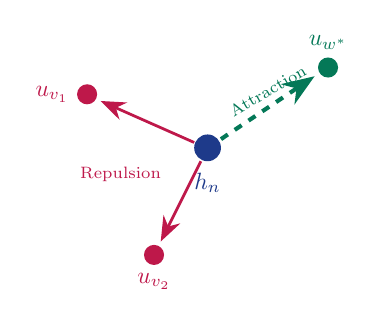
\begin{tikzpicture}[scale=0.85, every node/.style={transform shape}]
                % Center Node (h_n)
                \fill[primary] (0,0) circle (0.2) node[below=0.25cm, color=primary, font=\bfseries] {$h_n$};
                
                % Target Node (u_w*)
                \fill[accentgreen] (1.8, 1.2) circle (0.15) node[above=0.15cm, color=accentgreen] {$u_{w^*}$};
                \draw[accentgreen, -{Stealth[scale=1.2]}, dashed, line width=1.5pt] (0.2, 0.13) -- (1.6, 1.07);
                \node at (0.9, 0.85) [color=accentgreen, font=\scriptsize, rotate=30] {Attraction};
                
                % Repelled Node 1 (u_v1)
                \fill[accentpink] (-1.8, 0.8) circle (0.15) node[left=0.15cm, color=accentpink] {$u_{v_1}$};
                \draw[accentpink, {Stealth[scale=1.2]}-, line width=1pt] (-1.6, 0.7) -- (-0.2, 0.08);
                
                % Repelled Node 2 (u_v2)
                \fill[accentpink] (-0.8, -1.6) circle (0.15) node[below=0.15cm, color=accentpink] {$u_{v_2}$};
                \draw[accentpink, {Stealth[scale=1.2]}-, line width=1pt] (-0.7, -1.4) -- (-0.1, -0.2);
                \node at (-1.3, -0.4) [color=accentpink, font=\scriptsize] {Repulsion};
            \end{tikzpicture}
        \end{column}
    \end{columns}
\end{frame}

\begin{frame}{7. Conclusion \& Distributional Semantics}
    \begin{block}{Distributional Hypothesis Emergence}
        Semantic substitutions receive identical updates from shared contexts, settling the embedding space into a coordinate system where spatial proximity mirrors semantic overlap~\cite{harris_distributional_1954}:
        $$\cos(\theta_{w_1, w_2}) \to 1 \iff \mathcal{C}_{w_1} \approx \mathcal{C}_{w_2}$$
        where $\mathcal{C}_w$ represents the distribution of contexts in which token $w$ appears.
    \end{block}
    
    \vspace{0.1cm}
    \textbf{Summary:} The Transformer acts as a Bayesian engine where:
    \begin{itemize}
        \item \textbf{Attention \& FFNs} synthesize the context vector $h_n$.
        \item The \textbf{magnitude} $\|h_n\|$ models certainty as inverse temperature $\beta$.
        \item The \textbf{orientation} matches correlation $r$ with self-organized embeddings.
    \end{itemize}
\end{frame}

% Slide 9: References
\begin{frame}{References}
    \begin{thebibliography}{99}
        \tiny
        \bibitem{vaswani2017attention} Vaswani, A. et al. (2017). Attention is all you need. \textit{NeurIPS}.
        \bibitem{jaynes1957} Jaynes, E.T. (1957). Information theory and statistical mechanics. \textit{Phys. Rev.}
        \bibitem{geva-etal-2021-transformer} Geva, M. et al. (2021). Transformer feed-forward layers are key-value memories. \textit{EMNLP}.
        \bibitem{gao2019representation} Gao, J. et al. (2019). Representation degeneracy problem in training NLG models. \textit{ICLR}.
        \bibitem{ba2016layernorm} Ba, J.L. et al. (2016). Layer normalization. \textit{arXiv:1607.06450}.
        \bibitem{ackley1985learning} Ackley, D.H. et al. (1985). A learning algorithm for Boltzmann machines. \textit{Cognitive Science}.
        \bibitem{shannon1948mathematical} Shannon, C.E. (1948). A mathematical theory of communication. \textit{Bell Sys. Tech. J.}
        \bibitem{harris_distributional_1954} Harris, Z.S. (1954). Distributional structure. \textit{Word}.
    \end{thebibliography}
\end{frame}

\end{document}
